
In traditional datacenters, the practice is to either follow
a dedicated model and provision servers for peak loads, or share
resources in a best-effort manner that offers no
guarantees~\cite{resource-overbooking}.
For example, an auction website may be hosted on a single PM
in order to guarantee that it has enough resources to face peak loads.
However, this
results in under-utilization of resources and wastage of power during
low loads, say, when the auction website is idle during night.
Alternatively, co-hosting the auction website with another service 
in simply a
best-effort manner will be insufficient when either of the
co-hosted services is bombarded with heavy load.
Resource utilization can be maximized while still ensuring performance
guarantees through dynamic resource provisioning~\cite{sandpiper, 
vm-multiplexing}, by adopting virtualization
and consolidating/co-hosting multiple services (like
auction websites and email servers) as VMs on the same physical
machine~\cite{entropy}.

Several to-be-virtualized applications have data dependencies
between each other or among their components.
Example instantiations are, (i)~a multi-tier web-based application has
exchange of data
between its components\textemdash{}web-server, application logic server
and the database, and 
(ii)~heavily parallelized applications~\cite{high-consuming-parallel}
which have distributed computing tasks with mutual data dependencies.
\textit{Server consolidation} refers to mapping a set of applications/servers
to instances hosted within
virtual machines, in such a way as to maximize the utility of the
available infrastructure~\cite{load-balancing}.
Thus, server consolidation can facilitate sharing of available resources
among the tiers of a single application or 
across tiers of multiple applications,
using dynamic resource allocation and virtual machine
migration techniques~\cite{sandpiper, adaptation-engine}.


\begin{figure}[h]
	\centering
	\subfloat[Before Consolidation]{\includegraphics[height=4cm,width=5cm]{figures/before_consolidation.eps}}
	~~~~~~~~~~~~~~~~~~~~~~~~
	\subfloat[After Consolidation]{\includegraphics[height=4cm,width=5cm]{figures/after_consolidation.eps}}
\caption{Server Consolidation, via Virtualization, for efficient resource multiplexing.}
\label{virtualization-enables-consolidation}
\end{figure}

An example consolidation scenario is shown in Fig.~\ref{virtualization-enables-consolidation}, 
where two virtualized server instances are moved to or co-hosted on a single physical machine 
such that only one physical machine is sufficient to host both services and
the other machine which becomes idle can be powered off.
In the ``Before Consolidation'' case of Fig.~\ref{virtualization-enables-consolidation}(a), 
each physical machine is executing a single lightly-loaded virtual machine each. 
Here, power is being wasted in keeping both physical
machines ON though under-utilized. In the ``After Consolidation'' case,
both VMs have been moved to one of the physical machines. 
If both the VMs and the corresponding virtulization overheads can be accommodated
on a single PM,
the other resultant unused PM can be switched OFF. Such consolidation and
powering off of unnecessary resources results in better resource
utilization and saves copious amounts of power
(otherwise used for supplying power to machines as well as for cooling) in
the data-center.

\underline{Colocated and dispersed VMs:} When applications are 
instantiated in a virtual
environment, two major factors affect their performance\textemdash{}available
network capacity and virtualization-related CPU overhead,
and these factors vary based on whether the communicating VMs
are located on the same host or on different hosts~\cite{virtual-putty}.
\emph{Colocated}\index{Colocated} 
virtual machines (VMs\nomenclature{VM:}{Virtual machine}\index{VM} 
hosted on the same PM\nomenclature{PM:}{Physical machine}\index{PM}) incur 
different virtualization overheads for mutual network
communication as opposed to \emph{dispersed}\index{Dispersed} VMs 
(VMs placed on different PMs).
It is claimed in \cite{virtual-putty} that transitioning
between colocated and dispersed placements for communicating VMs
can result in a change in their CPU requirements. However, empirical
quantification is lacking.

\underline{Network affinity:} In general, VMs are said to have
\textit{network-affinity}
%\nomenclature{Network-affinity:}{Two VMs have 
%\textit{network-affinity} if they have network communication with each other.}
for each other if they have 
network communication between them~\cite{virtual-putty, starling}.
When VMs are colocated, the network traffic between them
is defined as being \textit{intra-PM}, whereas when they are dispersed,
it is \textit{inter-PM} network traffic.
Since migration of a VM can potentially change the nature of network
traffic between being \textit{intra-PM} and \textit{inter-PM}, depending 
on the source and destination hosts for migration, we define this
as the \textit{mutable} nature of network affinity, as explained next.

\underline{Mutable nature of network affinity:} Given a set of VMs, some 
of which may have network communication with one another, every 
``communicating pair'' of VMs is said to have network affinity for each other.
A migration of any one VM can, but need not necessarily, cause the nature of
network traffic between a VM pair to change from being \textit{intra-PM}
to \textit{inter-PM}, or from being \textit{inter-PM} to \textit{intra-PM}.
For example, suppose there are 4 VMs hosted on 4 PMs, as illustrated
in Fig.~\ref{fig:mutable}(a). The VM pairs that have
network affinity are, (i)VM1 $\leftrightarrow$ VM2,
(ii)VM2 $\leftrightarrow$ VM3 and,
(iii)VM3 $\leftrightarrow$ VM4. 

\begin{figure}[h]
\begin{center}
	\subfloat[Initial configuration]{\includegraphics[scale=0.6]{arescue-figures/mutable-immutable.pdf}}
	~~~~~~~~~~~~~~~~~~~~~~~~~~
	\subfloat[VM3 migrates to PM2]{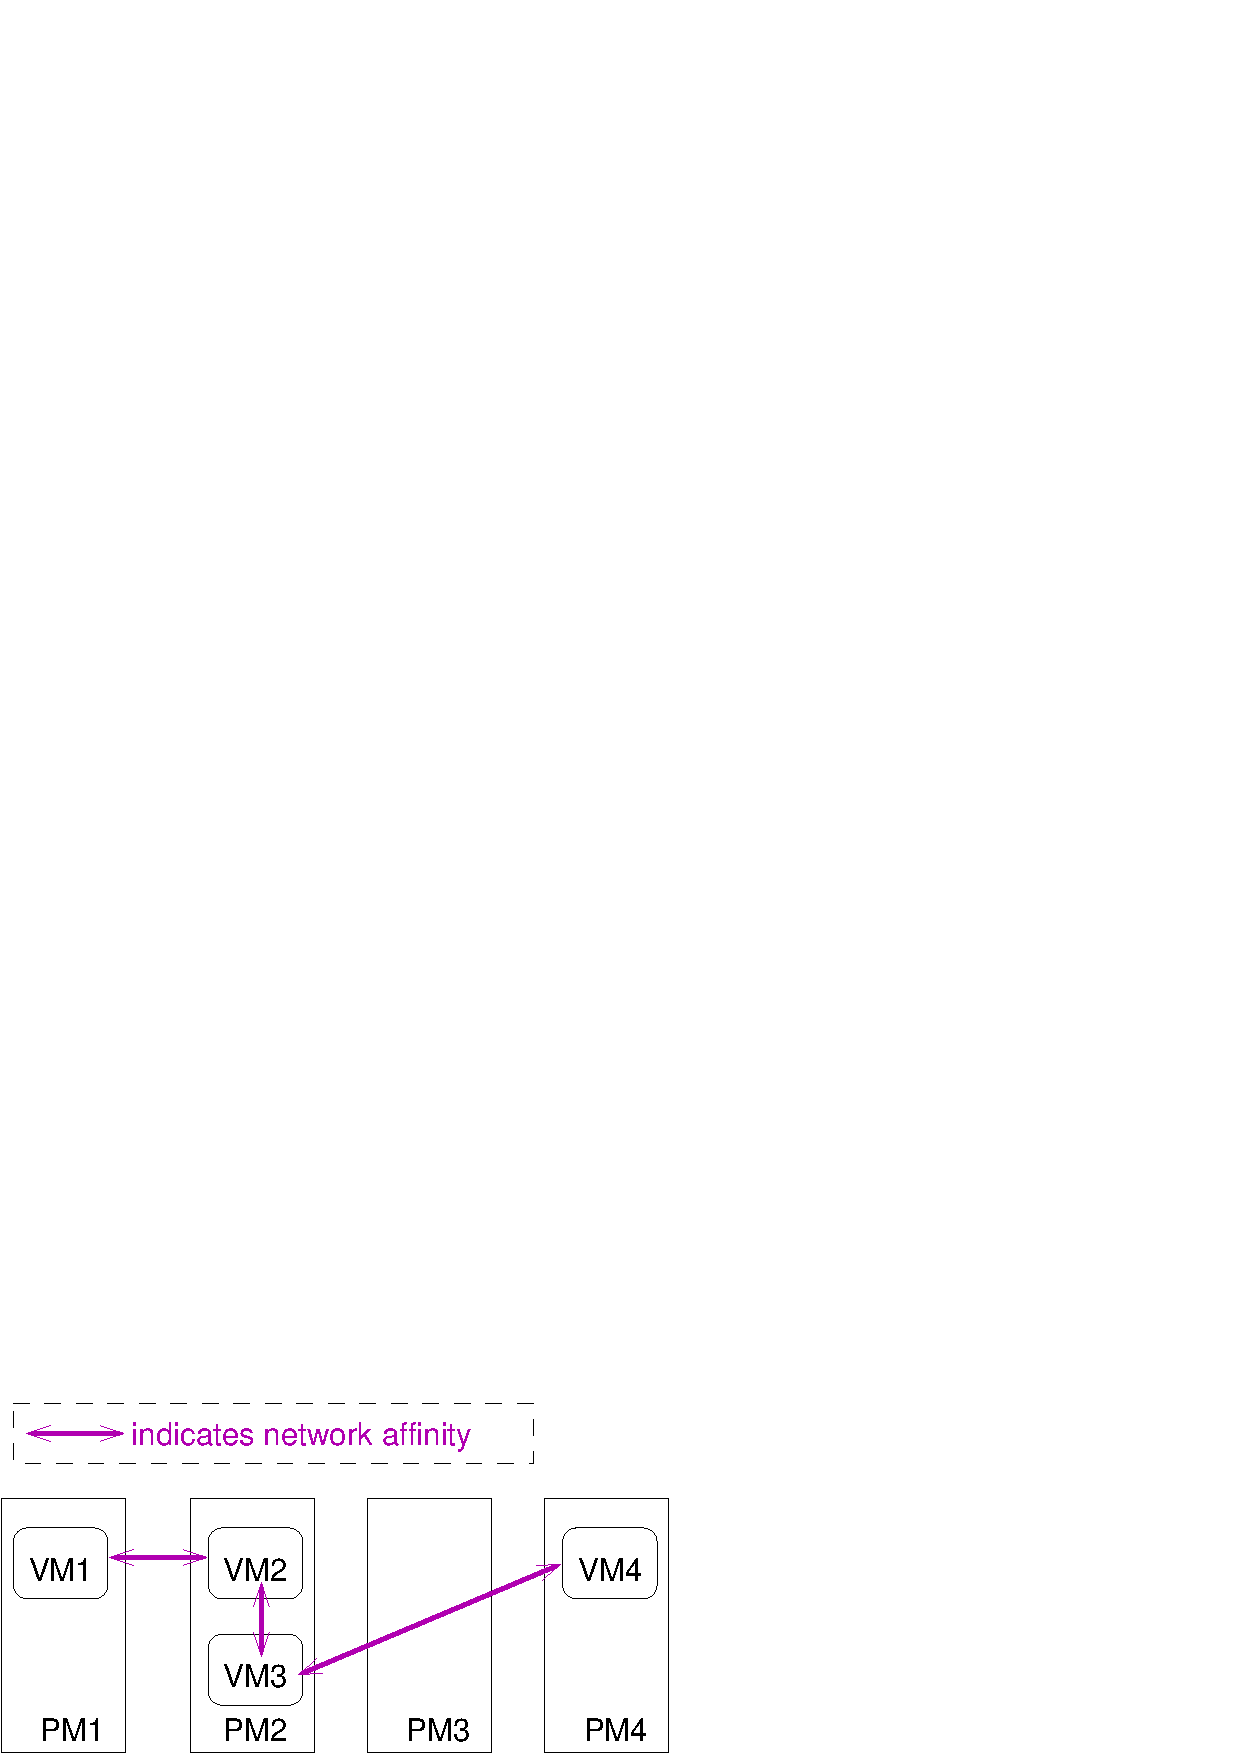
\includegraphics[scale=0.6]{arescue-figures/mutable-immutable-2.pdf}}
	\caption{Example to demonstrate \textit{mutable} and \textit{immutable} network affinity.}
\label{fig:mutable}
\end{center}
\end{figure}

In the initial state (refer Fig.~\ref{fig:mutable}(a)), all VMs are
hosted on different PMs (i.e. dispersed), hence the network traffic
in each case is \textit{inter-PM}. Suppose VM3 is now migrated from
PM3 to PM2, it gets colocated with VM2, resulting in the 
configuration shown in Fig.~\ref{fig:mutable}(b). 
After the migration, the nature of traffic between VM2 and VM3
has changed from \textit{inter-PM} to \textit{intra-PM}, whereas VM2
continues to have \textit{inter-PM} network affinity with VM1.
Thus, migration of VM2 caused its network traffic with VM3 to 
change nature, while its traffic with VM1 remained unchanged. We differentiate
these two types of network traffic as \textit{mutable} and \textit{immutable}
network traffic.
Basically, for a given VM migration, \textit{mutable} network traffic 
is that which changes nature between \textit{inter-PM} and \textit{intra-PM},
and \textit{immutable} network traffic is that whose nature does not change
due to the migration.

We present benchmarking experiments
which demonstrate impact due to network affinity
on CPU usage of virtual machines and their hosts, when communicating
VMs are colocated as compared to when they are dispersed. 
Motivated by the benchmark findings, we develop models
that can estimate the ``colocated'' CPU resource usage when VMs transition
from dispersed placements to colocated, and can estimate the ``dispersed''
CPU resource usage when VMs transition from colocated placements to dispersed. 
These models predict CPU usage in target
scenario (colocated/dispersed) based on resource usage profiles
from source scenario (dispersed/colocated).

Initially we built models to predict total CPU usage for target scenario,
based on all resource usage profiles like CPU, disk, mutable network
and immutable network usage. However, the maximum error with these
predictions was found to be around 4 to 6\% absolute CPU usage.
Consequently, based on our findings that CPU usage is affected only by
\textit{mutable} network traffic levels, we built models to
predict the difference in CPU usage based on only
the mutable network traffic profiles. These models were much more
accurate, with maximum error within 2\%. Finally, we applied these
pair-wise models to multi-VM scenarios using a multi-phase
prediction methodology. This demonstrated that simple models
built on the scale of two VMs could be successfully used to
predict for multi-VM scenarios as well.
%In our work, we perform empirical quantification of 
%the CPU resource that Xen-based VMs would require if they were
%to be migrated for colocation or dispersion (splitting up of 
%previously-colocated VMs). 
%
%We are concerned with CPU utilization required to handle network
%In Xen virtualization environment, a
%privileged virtual machine (called Domain-0 or 
%Dom0\index{Dom0}\nomenclature{Dom0:}{Privileged domain or privileged virtual 
%machine or Domain-0}) manages network 
%traffic for the guests (called User Domain or 
%DomU\index{DomU}\nomenclature{DomU:}{User domain or Domain-U})
%and utilizes CPU proportional to network traffic volume.
%In this work, we explore the effect of
%network-affinity on CPU usage of colocated and dispersed VMs. More
%specifically, \textit{what is the effect on CPU utilization of mutually
%communicating VMs based on whether they are colocated or dispersed?}
%An important consideration for migration and consolidation related
%decisions is the expected resources required for the VM
%on the target machine. The consolidation of
%VMs into a colocated set and the migration of VMs to dispersed
%placements, can result in different CPU resource requirements.
%The focus of the first component of this thesis, is to build
%\emph{affinity-aware} models that can predict expected CPU
%resource requirements\textemdash{}upon colocation or dispersion of VMs.
Our contributions are,
\begin{enumerate}	
\item \emph{Event profiling} of intra-PM and inter-PM network
	communication paths in Xen, using \texttt{Xenoprof}~\cite{xenoprof}.
\item \emph{Benchmark} CPU resource requirements
of VMs with different levels of network-affinity
in colocated and dispersed configurations.
\item Perform the above benchmarking step for both Xen and KVM virtualization environments,
	showing that a linear relationship between network usage and the resulting CPU overhead
	exists in both.
\item Develop \emph{pair-wise affinity-aware} models to predict \textit{total}
	as well as \textit{differential} CPU usage, when a pair of VMs move between
	dispersed and colocated placements.
\item Apply above pair-wise models to \emph{multi-VM scenarios}, where
	a single migrating VM has more than one neighboring
	VMs with which it exhibits network-affinity, both on source \& target PMs.
\item Present a \emph{comprehensive evaluation} using synthetic 
	workloads \& benchmark applications,
	of the pair-models as well as application to multi-VM scenarios.
\end{enumerate}

\noindent The rest of this chapter is structured as follows. 
Section~\ref{sec:arescue-background}
presents background regarding network virtualization in Xen and KVM, and
problem statement is presented in Section~\ref{sec:arescue-problem}.
Section~\ref{sec:arescue-benchmark}
presents empirical benchmarking of the effects of relative placement on
CPU usage of communicating VMs, in both Xen and KVM virtualization environments.
Section~\ref{sec:arescue-our-approach} presents our approach to
build affinity-aware models to predict CPU usage for Xen DomU and Dom0
and Section~\ref{sec:arescue-experimental-eval} presents evaluation 
of the models.
Section~\ref{sec:arescue-related-work} presents related work in juxtaposition
with our work and 
in Section~\ref{sec:arescue-open-directions}, we
present our ideas for future work.
%in the area of affinity-aware CPU usage modeling and 
Section~\ref{sec:arescue-conclusions} concludes the chapter.

